\documentclass[12pt,a4paper,twoside]{article}
\usepackage[latin1]{inputenc}
\usepackage{amsmath}
\usepackage{array}
\usepackage{amsfonts}
\usepackage{amssymb}
\usepackage{afterpage}
\usepackage{hyperref}
\usepackage{tocloft}
\usepackage{pifont}
\usepackage{graphicx}
\graphicspath{{../Matlab/Figures/}}
\usepackage{subcaption}
\renewcommand{\baselinestretch}{1.1}
\renewcommand{\cftsecleader}{\cftdotfill{\cftdotsep}} % for sections
\usepackage{hyperref}
\usepackage[left=1in, right=1in, top=1in, bottom=1in]{geometry}
\author{Giammario Fulco [191071]\\
\texttt{giammario.fulco@studenti.unitn.it}}
\title{\textbf{Vibration Mode Analysis}\\
	Course project\\
	Systems and Techniques for Digital Signal Processing\\}
\let\oldsection\section
%\def\section{\cleardoublepage\oldsection}
%
%\usepackage{draftwatermark}
%\SetWatermarkLightness{0.9}
%\SetWatermarkScale{5}
%
\begin{document}
\vspace{-1em}
\maketitle
\vspace{-2em}
\tableofcontents
\thispagestyle{empty}
\afterpage{\pagestyle{empty}}
%\clearpage
\thispagestyle{empty}
~
\clearpage
\setcounter{page}{1}
%
\section{Introduction}
This project will cover the topic of analyzing Modes of vibration of a Clamped Beam subjected to an external force. 3 accelerometers placed in different positions of the beam, supposedly where the modes of vibration are maximum, will acquire data of the beam's movement and provide the data for the analysis. The Matlab simulation platform will be the tool used to perform the analysis and draw the plots.\\

\begin{figure}[h!]
	\centering
	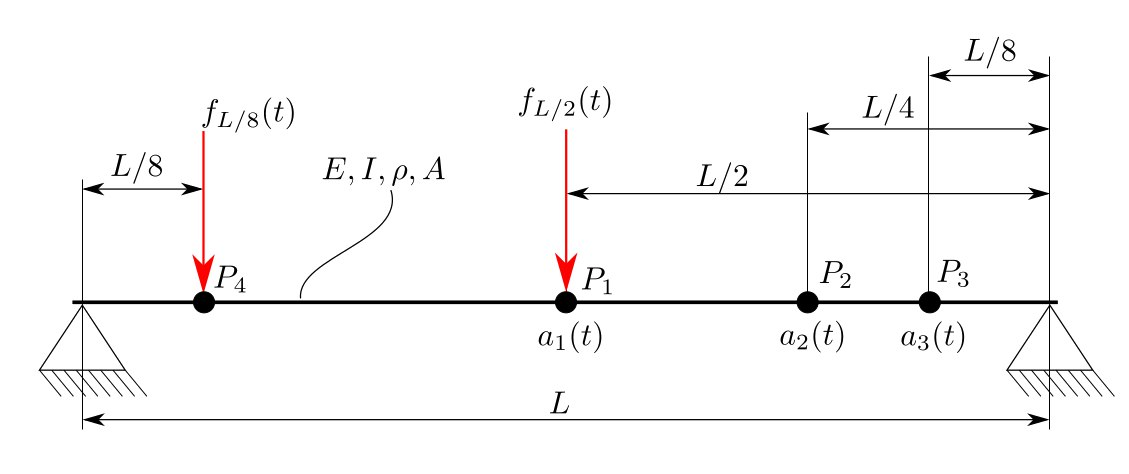
\includegraphics[width=0.9\linewidth]{Images/beam.jpg}
	\caption{Analytical model and accelerometers position.}
	\label{beam}
\end{figure}
\noindent

The analysis parameters are:
\begin{itemize}
	\item Time Interval: 10 s.
	\item Sampling Frequency: $10240$ Hz.
	\item Filter applied to the data: Low-pass Butterworth Filter.
	\item Cut-Off Frequency: $5$ KHz.
	\item Number of Acquisitions: 4
\end{itemize}
\bigskip \bigskip \bigskip \bigskip \bigskip \bigskip
\bigskip
\bigskip
\bigskip
\section{Impulse and Frequency Responses}
\subsection{Impulse Response}
First step to have a good vibration mode analysis is computing and visualizing the impulse response of the system. Since the input force in our case can be seen as an approximation of an ideal impulse, the data acquired by the accelerometers can be seen as the impulse response of our system as shown in \figurename{ \ref{forces}}. In \figurename{ \ref{forcespart}} the zoom plot is shown to underline the difference between the real impulse, which is the one analyzed in this relation and an ideal one which is a Kronecher delta.\\

\begin{figure}[h!]
	\centering
	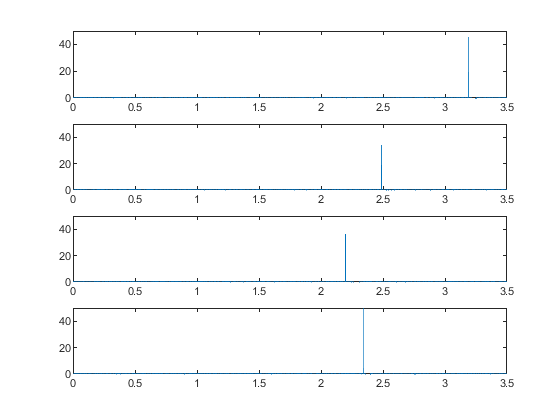
\includegraphics[width=0.9\linewidth]{Images/forces.png}
	\caption{Forces plot for each instance.}
	\label{forces}
\end{figure}
\noindent

\begin{figure}[h!]
	\centering
	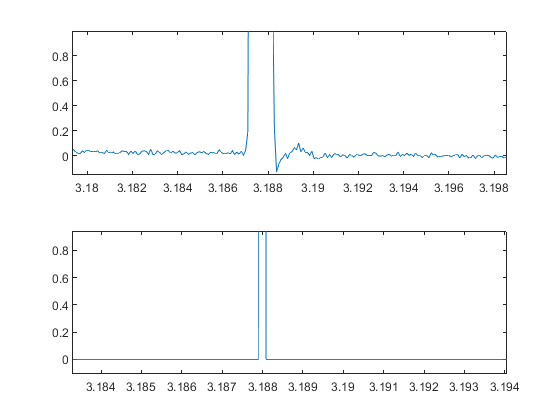
\includegraphics[width=0.9\linewidth]{Images/delta.png}
	\caption{Differences between real impulse and Ideal one.}
	\label{forcespart}
\end{figure}
\noindent

Then the impulse response of the beam system will be shown in \figurename{ \ref{meanimp}}. To avoid overloading the relation with images, just the mean impulse response for each accelerometer will be shown. Since the impulse applied is very short, the most important part of the response is concentrated at the beginning of the signal, so the plot will show the first 0.1 seconds of the impulsive response.

\begin{figure}[h!]
	\centering
	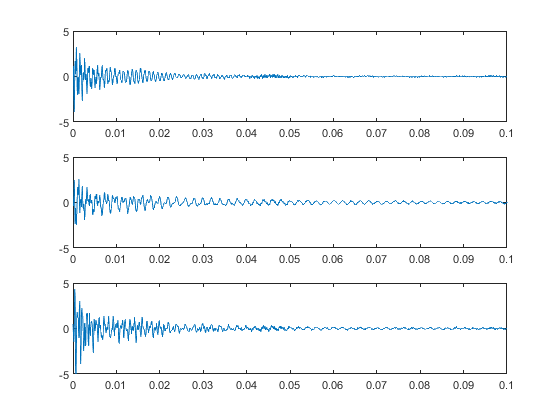
\includegraphics[width=0.9\linewidth]{Images/meanimp.png}
	\caption{Mean Impulse response of the accelerometers.}
	\label{meanimp}
\end{figure}
\noindent

\subsection{Frequency response}
Next step in the vibration mode analysis is to get the frequency response of the system. From theory we know that it is defined as the Fourier transform of the impulsive response.
\begin{equation}
	H(e^{j\omega}) =\sum_{-\infty}^{+\infty}h(n)e^{-2\pi j \omega n}
	\label{Qn}
\end{equation}

Matlab provides various tools to perform the Discrete Time Fourier transform of a signal. Most efficient computationally speaking is the Fast Fourier Transform (FFT), which is a collection of algorithm that aims to lower the burden of performing complex multiplication and addition, which are necessary in the Fourier transformation. One thing that can be noticed is that since we are sampling the signal at $$f_s = 10240 Hz$$ and the sampling time is $T = 10 s$ we will have a total number of samples of $$ N = 102400 $$ This is important because one of the characteristics of FFT algorithm is that it reach the maximum computational efficiency when the number of samples N used for the transformation is a power of 2, namely:
$N = 2^{\nu}$ with $ \nu \in N$. It's easy to see that since $log_2 102400 = \nu \not\in N $ then the number of samples in our experiment has not an optimal number of samples. Luckily enough, Matlab offers a solution for this issue, for algorithm performance purposes, fft() function allows the user to pad the input with trailing zeros. In this case, pad the signal with zeros so that the length is the next higher power of 2 from the current length. Define the new length using the nextpow2() function. Since this analysis is performed offline with a priori collected data and not online with live data acquisition the performance of the algorithm is not a critical parameter. Then the signal is not padded in this case, but it was worth examining the problem.
Now we can show the frequency response of the system, same way as the impulse responses, only the mean frequency response will be shown keeping in mind that in the following sections we will work with frequencies in the range [0 2000] Hz. 
\begin{figure}[h!]
	\centering
	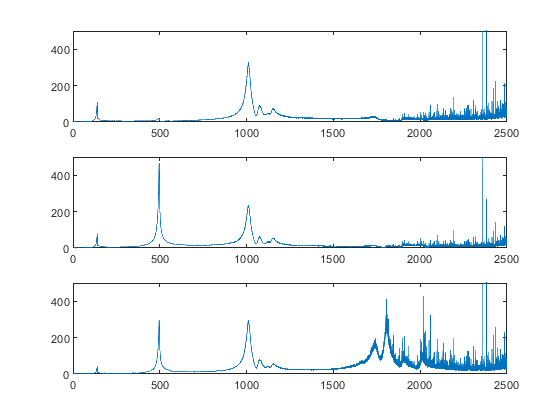
\includegraphics[width=0.9\linewidth]{Images/meanfreq.png}
	\caption{Mean frequency response of the accelerometers. $|H(e^{j\omega})|$}
	\label{meanfreq}
\end{figure}
\noindent


In \figurename{ \ref{meanfreq}} the  absolute value of mean frequency response, up to 2500 Hz of each accelerometer, is shown. As said in Section 1, sensors are positioned in the presumed position of maximum amplitude of a vibration mode. That is why we can see that in each of the plots the amplitude of one of the modes is higher with respect to the same mode's amplitude in the other plots. We can also notice that a Vibration mode around 1800 Hz is present only in one of the frequency responses. That happens because the first and second accelerometer are placed on a Node of that specific mode of vibration, in other words, the component of the last mode of vibration is 0 in the positions where the accelerometer 1 and 2 are placed.



\bigskip \bigskip  

\section{Modes of Vibration Analysis}
Once the frequency responses are computed, next step is analyzing the spectrum of the signal to find significant data.
\subsection{Frequency responses Peaks}

The peaks of the absolute value of the frequency responses indicates the frequency at which the beam system is vibrating. Even though Matlab has a built in function to retrieve peaks of a signal which is called findpeaks(), for this relation, a custom routine has been written to find the maxima of the single sided spectrum. The function called peaks(), allows the user, once given the signal and the frequency axis as inputs, to pass as further input parameters some assumption on the position, width and distance between one peak and another as well as the maximum desired frequency for the peaks in order to get position of the maxima. Basically the function will spot the points where the derivative of the frequency response (in absolute value) changes in sign and using these points as reference, since in the maxima points the derivative is null, starting from the bigger in value, the function sets a portion of the frequency response to 0. Then the function iterates over a set number of maximum decided by the user. Since the signal is noisy,  to smooth the searching operation a moving average filter is applied to the signal. In \figurename{ \ref{confronto}} it's shown how the moving average will smooth the signal in exchange for a reduction in amplitude of the peaks. Once the peaks have been found, a range around the smoothed peak is saved and then the real amplitude and position can be retrieved from the raw signal using the built-in matlab function max().

\begin{figure}[h!]
	\centering
	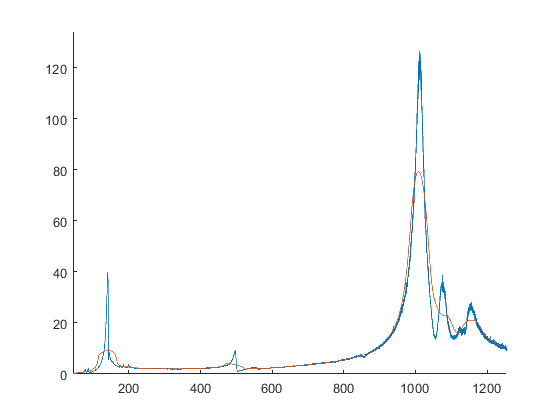
\includegraphics[width=0.8\linewidth]{Images/confronto.png}
	\caption{Frequency response vs Filtered Frequency response}
	\label{confronto}
\end{figure}
\noindent

In \figurename{ \ref{peaks}} we can see the results of this approach. A final comment on this procedure is on the length chosen for the Moving average period. Since a period that is too high will lead to a lag in the response and a consequential error in the range where the max() function is getting applied, by a trial and error process, a length $L_{ma} \tilde{=} 1/20 L$ has been chosen.

\begin{figure}[h!]
	\centering
	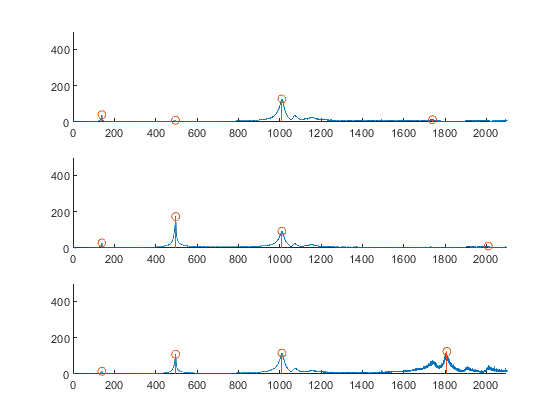
\includegraphics[width=0.8\linewidth]{Images/peaks.png}
	\caption{Peaks for one instance of each accelerometer}
	\label{peaks}
\end{figure}
\noindent

%
\subsection{Statistical moments of the peaks}

In this section we will tackle on the steps to make a statistical analysis of the position and amplitude of the previously identified peaks. In particular we will find the mean value and the standard deviation for the maxima amplitude and position.
We can give a brief recall on the definition of mean value and standard deviation before starting. Mean value of a collection $x$ is defined as $$\mu_{x}= \frac{1}{N} \sum_{i=1}^{N} x_{i}  $$
While its (corrected) standard deviation is defined as
$$ \sigma_{x} = \sqrt{\frac{1}{N-1}\sum_{i=1}^{N}(x_{i} - \mu_{x})^{2}}$$
The corrected version differs in the usage of $\frac{1}{N-1}$ instead of $\frac{1}{N}$ because the mean value is obtained through a small sample.
In \figurename{ \ref{meanpeaks}} we can see the overlapping of the mean frequency response and the mean value found for position and amplitude of the maxima.

\begin{figure}[h!]
	\centering
	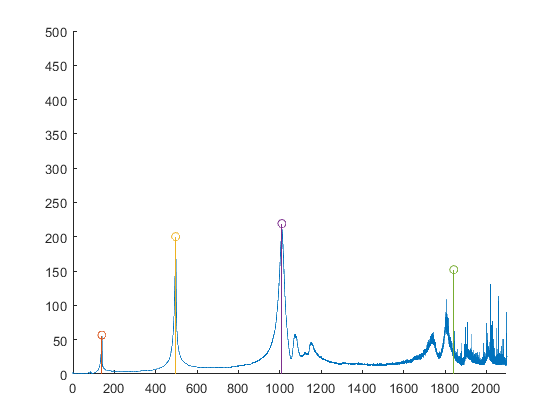
\includegraphics[width=0.8\linewidth]{Images/meanpeaks.png}
	\caption{Mean Peaks and Mean Freq response overlapping}
	\label{meanpeaks}
\end{figure}
\noindent

While in  \figurename{ \ref{stdpeaks}} we can see a zoom version of the previous plot which also include the standard deviation for a single peak to have a better visualization.
\begin{figure}[h!]
	\centering
	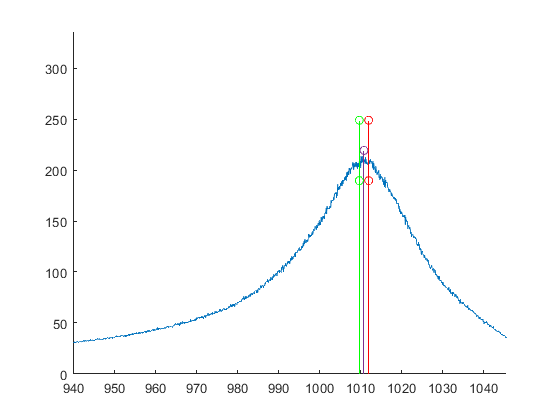
\includegraphics[width=0.8\linewidth]{Images/stdpeaks.png}
	\caption{Standard deviation range particular.}
	\label{stdpeaks}
\end{figure}
\noindent

The most important thing to notice by looking at \figurename{ \ref{peaks}} and \figurename{ \ref{meanpeaks}} is that the algorithm fails to retrieve a correct position and amplitude for the highest frequency peak. This is due to the position of 2 accelerometers which as said before are placed on a node of the specific frequency but also due to the not optimal performance of the peaks() function which is in charge of retrieving the peaks as well as the higher noise content at high frequency of the frequency response. This is shown very well by the standard deviation value of the last maximum point, which results to be 2 orders of magnitude higher than the previous three.

\section{Filter Design}

In this section, we will proceed to design a set of Notch filters that will have the function of attenuate the frequency at which the beam is vibrating.

\subsection{Notch Filters}

In signal processing, a band-stop filter is a filter that passes most frequencies unaltered, but attenuates those in a specific range to very low levels. It is the opposite of a band-pass filter. A notch filter is a band-stop filter with a narrow stopband (high Q factor).
To create the filters a simple routine has been written which allows the user to create a FIR notch filter using the windowing method.
Basically the routine takes as input the stopband frequency and creates an ideal filter which will then be windowed following criteria specified in the other parameters which are, and the width of the ideal notch filter, the length of the window and the type of window, chosen between rectangular, triangular and Gaussian.
In this section the results achieved with this approach will be shown and a brief explanation will be given for the choices made in the design of the filter parameters.
First of all, the choice of a FIR filter is made because it has a set of interesting properties, which are:
\begin{itemize}
    \item Inherent Stability
    \item Linear Phase easily achievable
\end{itemize}

The downside is that the computational load is higher on general purpose processor with respect to IIR filters, but again, since the data are collected a priori and not processed online that choice fits better the purpose of this work.
Next choice to discuss is: why use the windowing method?
The main reason is that is the simplest way to design a FIR filter, since there were no specification given on how to design the passband and stopband tolerances. The resulting tolerances will be equal in stop and pass band and there will be an unnecessary high accuracy in the passband, which is not completely a drawback. In any case this filter will NOT be the optimal one in the sense of complexity order and delay. To design the optimal FIR filter for the case, specification in the passband and stopband are needed and an iterative process is required.
The possible windows chosen for the experiment are respectively, rectangular and triangular(Bartlett) which are the simplest possible windows described during the lecture and Gaussian which has been chosen because it was not introduced during the course and could be a good learning example. There are better windows (cosine class windows) that could give better results since they have better approximation error and magnitude ratio between main lobe and side lobes, although they have worst frequency resolution for a fixed length the cut off frequency for the filters' set we are going to design are pretty far apart from each other. Overall this class of windows would have been the best choice to address this problem, to keep the experiment simple, the above mentioned windows have been chosen. Moreover, the implementation of different windows within the notchfilter() function can be easily done with few code lines, since the procedure has been designed to be scalable.
At this point, the width of the ideal notch filter has to be picked, assuming, as confirmed by literature, that notch filters have usually 1 to 2 decades stopband width, the highest frequency attenuated is 10 times the lowest frequency attenuated, which means one decade or in numbers: $$ W = \frac{11}{18} \omega_{peak}$$
As for $\omega_{peak}$ the choice is easily made by picking the mean value found in the previous section.
At last, the Length of the window needs to be choosen. From the course theory, we know that chosing the Length L impacts on the frequency resolution in combination with the width of the main lobe. For example with a rectangular window we will have that:
$$ \Delta_{\omega} = \frac{1}{t_{window}}$$
Meanwhile with a Triangular window: 
$$ \Delta_{\omega} = \frac{2}{t_{window}}$$
This basically means that increasing the length of the window improves the capability of distinguish two different frequency.
Improving the length as also some downsides, the time resolution degrades and the computational time increases.

\subsection{Results}

Now the procedure for the windowing method and related graphs, will be shown. Using the previously established parameters, let's try to design a notch filter for the first peak of the transfer function. Removing following peaks would just be a mere iteration of the following process.
Then let us pick the mean value of the first pick for the desired stopband frequency $\omega_{p} $and correspondely to what has been said before $\frac{18}/{11} \omega_{p}$ for the width of the ideal filter. A Gaussian window will be picked with a length $L = 500$ which is about $\frac{1}{10}$ of the Single sided spectrum length.
First step consists in building the ideal filter which is shown in \figurename{ \ref{idealnotch}} since we want a real impulsive response, we have to be sure that the frequency response is symmetric.

\begin{figure}[h!]
	\centering
	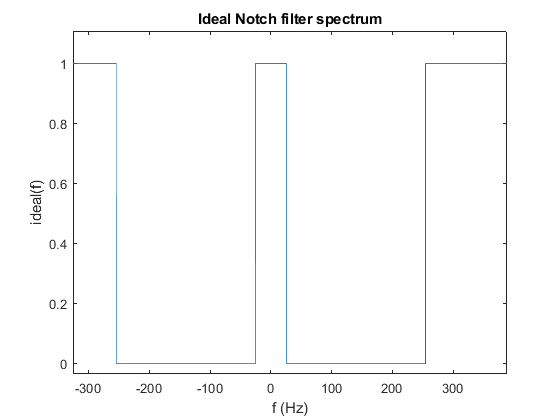
\includegraphics[width=0.8\linewidth]{Images/idealnotch.png}
	\caption{Ideal notch filter frequency response}
	\label{idealnotch}
\end{figure}
\noindent

Next step is using the Inverse Fourier Transform inbuilt function of Matlab to get the ideal impulse response. In \figurename{ \ref{idealnotchimp}} the behaviour of the filter in the time domain is shown.

\begin{figure}[h!]
	\centering
	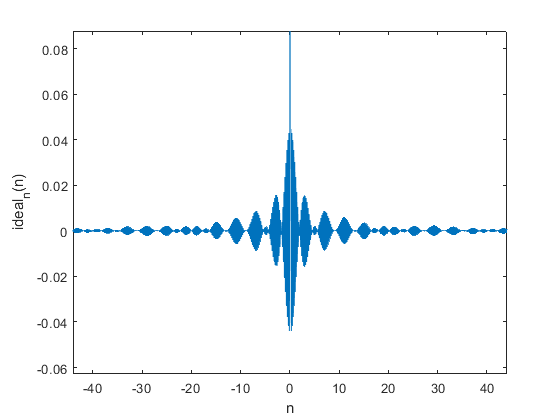
\includegraphics[width=0.8\linewidth]{Images/idealnotchimp.png}
	\caption{Ideal notch filter impulse response}
	\label{idealnotchimp}
\end{figure}
\noindent

The windowing method consists in using the already defined ideal impulse response and use and applying a window to it. Since we decided to use a Gaussian Window, in \figurename{ \ref{gauss}} this window is shown. 


\begin{figure}[h!]
	\centering
	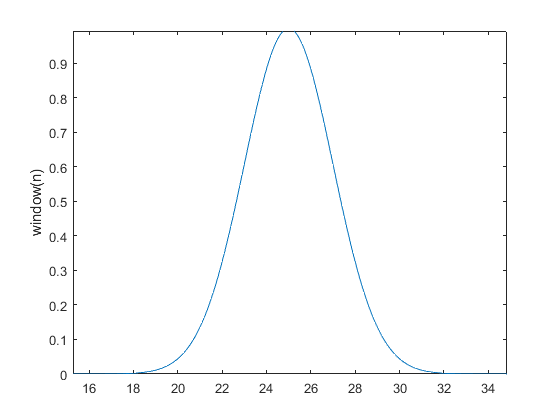
\includegraphics[width=0.8\linewidth]{Images/gauss.png}
	\caption{Causal Gaussian window of length L}
	\label{gauss}
\end{figure}
\noindent

From the theory we know that we can apply the window in the time domain by multiplying the ideal impulse response and the window or applying the Windowing Theorem we can use the Ideal frequency response and the transformed window and apply a convolution in frequency.

$$h_{id}(n)w(n) = \frac{1}{2\pi}\int_{-\pi}^{\pi} H_{id}(e^{j\theta})W(e^{j(\omega - \theta))} d\theta $$

In this case, we will just multiply the signals in the time domain, although before performing the multiplication the ideal impulse response must be shifted of $frac{L}{2}$ samples to have a causal behaviour. The time domain windowed filter is shown in \figurename{ \ref{windowed}} The fact that the new impulse response is limited in time and the side lobes are smaller due to the windowing is clearly seen in the picture.

\begin{figure}[h!]
	\centering
	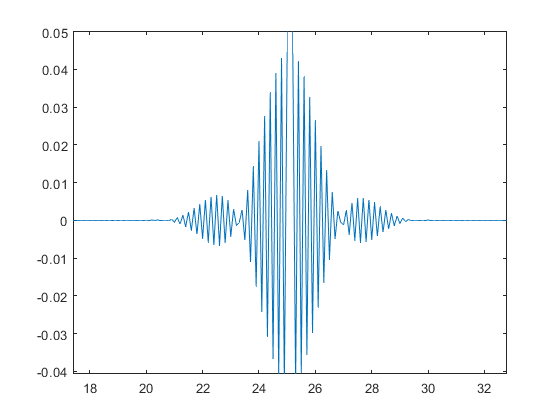
\includegraphics[width=0.8\linewidth]{Images/windowed.png}
	\caption{Windowed Impulse response}
	\label{gauss}
\end{figure}
\noindent

Last step in the filter design process is to transform the impulse response in the frequency domain to have the final frequency response of the filter which is shown in \figurename{ \ref{filterresp}}

\begin{figure}[h!]
	\centering
	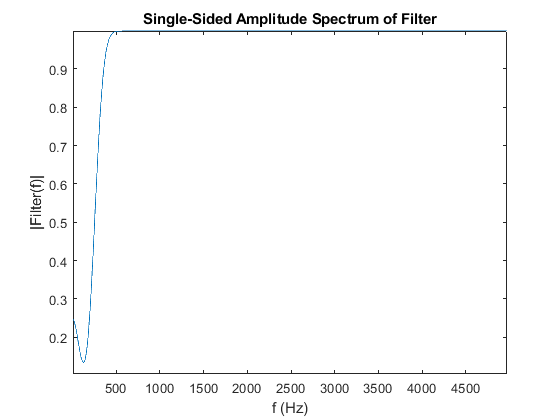
\includegraphics[width=0.8\linewidth]{Images/filterresp.png}
	\caption{FIR filter frequency response}
	\label{filterresp}
\end{figure}
\noindent

At last, let's show how the filter works, comparing the filtered frequency response with the non filtered one. In  \figurename{ \ref{compare}} the comparison is shown, with the zoom is clearly visible how the vibration mode frequency is highly attenuated while in about a decade before and after the peak the 2 frequency response will coincide again. This proves that the filter works well, but since the window used is really simple is difficult to see the effect of spectral leakage which is present for sure in this kind of filter. Possible improvements, except the already discussed possibility of having more windows type is for sure the possibility of plotting the zero/pole diagram of the filter which would require a symbolic definition of the filter.


\begin{figure}[h!]
	\centering
	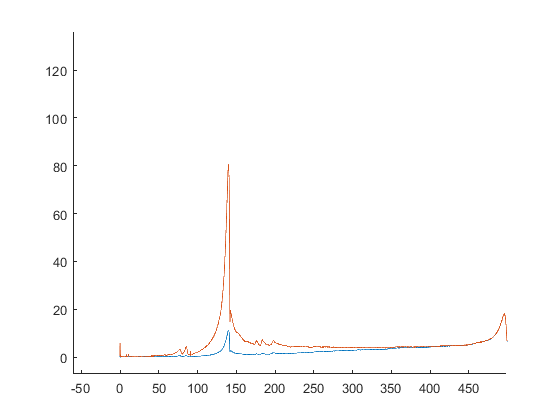
\includegraphics[width=0.8\linewidth]{Images/comparison.png}
	\caption{Filtered vs Non filtered response}
	\label{compare}
\end{figure}
\noindent


\end{document}